\section{A star of cold, non-interacting fermions}
\label{section: cold fermi star}


Ekstra kilder: \autocite{andersenIntroductionStatisticalMechanics2012,glendenningCompactStarsNuclear2012}
\todo{Ha kilder på riktig sted}

\todo{Skrive om white dwarfs/neutron stars?}
A non-interacting Fermi gas is governed by the Dirac Lagrangian
%
\begin{equation}
    \Ell = \bar \psi (i \slashed \partial - m) \psi,
\end{equation}
%
as described in (APPENDIX thermal field theory).
\todo{add appendix}
In the grand canoncial ensamble, the density of a conserved charge is regulated by a chemical potential $\mu$.
The conserved current corresponding to the $\text U(1)$ phase symmetry of the Dirac Lagrangian, i.e., the transformation $\psi \rightarrow e^{i \alpha} \psi \approx 1 + \alpha \delta \psi$, is
\begin{equation}
    j^\mu = \diffp{\Ell}{(\partial_\mu \psi)} \delta \psi = \bar \psi \gamma^\mu \psi.
\end{equation}
%
The conserved charge is
%
\begin{equation}
    Q = \int \dd^3 x \, j^0 = \int \dd^3 x\, \bar \psi \gamma^0 \psi,
\end{equation}
%
the number of particles minus antiparticles.
The total energy $U$ is related to the grand canonical free energy $F$ by a Legendre transformation,
%
\begin{equation}
    F(T, V, \mu) = U - T S - \mu Q, \quad \dd F = - S \dd T - p \dd V - Q \dd \mu.
\end{equation}
%
Here, $p$ is pressure, $T = {1}/{\beta}$ is temprature, and $S$ entropy.
These thermodynamic variables are related to the free energy by
%
\begin{equation}
    S = - \diffp{F}{T} = \beta^2 \diffp{F}{\beta}, \quad
    Q = - \diffp{F}{\mu}, \quad
    p = - \diffp{F}{V}.
\end{equation}
%
When the free energy can be written as $F = V \Eff$, where the free energy density $\Eff$ is independent of the volume $V$, then $\Eff = - p$ and
%
\begin{equation}
    \dd (V \Eff) = V \dd \Eff - p \dd V,
\end{equation}
%
allowing us to write
%
\begin{equation}
    \Eff(T, \mu) = u - Ts - \mu n, \quad
    \dd \Eff = -s \dd T - n \dd \mu,
\end{equation}
% 
where $s$ and $n$ are entropy and charge density, defined by
%
\begin{equation}
    s = - \diffp{\Eff}{T} = \beta^2 \diffp{\Eff}{\beta}, \quad
    n = - \diffp{\Eff}{\mu}.
\end{equation}
%
With this, we can write the energy density as
%
\begin{equation}
    u = \diffp{}{\beta} \left(\beta \Eff\right) + \mu n.
\end{equation}



The free energy density of the Fermion gas is (REF: appendix felt teori)
%
\begin{equation}
    \Eff = - 
    \frac{2}{\beta}\int \frac{\dd^3 p}{(2 \pi)^3} 
    \left[
        \beta \omega
        +
        \ln\left(1 + e^{-\beta(\omega - \mu)}\right)
        + 
        \ln\left(1 + e^{-\beta(\omega + \mu)}\right)
    \right],
\end{equation}
%
where $\omega = \sqrt{p^2 + m^2}$.
The first term in the integral is the divergent vacuum energy, which must be renormalized.
We can drop this term; it does not have any observable effects on our results, as we are interested in relative pressure and energy density.
With this, we find the charge density
%
\begin{equation}
    n = \frac{1}{\pi^2} \int \frac{\dd^3 p}{(2 \pi)^3} [n_f(\omega - \mu) - n_f(\omega + \mu)],
\end{equation}
%
where
%
\begin{equation}
    n_f(\omega) = \frac{1}{e^{\beta \omega} + 1}.
\end{equation}
%
is the Fermi-Dirac distribution.
The energy density is 
%
\begin{equation}
    \label{energy density}
    u = \frac{1}{\pi^2} \int_0^\infty \dd p\, p^2 \, \omega \, [n_f(\omega - \mu) + n_f(\omega + \mu)].
\end{equation}
%
As expected, this is the energy per mode times the density of states, integrated over all modes.
To write the pressure, $p = - \Eff$ in terms of an integral over the Fermi-Dirac distribution, we integrate by parts.
We have
%
\begin{equation}
    \int_0^\infty \dd p \, p^2 \ln\left[1 + e^{-\beta(\omega \pm m)}\right]
    = 
    \frac{1}{3} p^3\ln\left[1 + e^{-\beta(\omega \pm m)}\right] \bigg |_0^\infty
    + 
    \frac{1}{3} \int_0^\infty \dd p \, \frac{ \beta p^4}{\omega}n_f(\omega \pm \mu),
\end{equation}
%
where the boundary term vanish.
This allows us to write the pressure as 
%
\begin{equation}
    \label{pressure}
    p = \frac{1}{3} \int_0^\infty \dd p \, \frac{p^4}{\omega} [n_f(\omega - \mu) + n_f(\omega + \mu)]
\end{equation}


\todo{les over dette avsnittet}
We are interested in the $T = 0$ limit.
In this case, the Fermi distribution becomes a step function, $n_f(\omega) = \theta(-\omega)$.
Without loss of generality, we assume that $\mu > 0$, i.e., we are dealing with an abundance of matter compared to anti-matter.
The dispersion relation $\omega = \sqrt{p^2 + m^2}$ is always positivive.
This means that the contribution to thermodynamic quantities from anti-particles vanish, as the integral is multiplied with $n_f(\omega + \mu) = \theta(-\omega - \mu)$, where the argument $-\omega - \mu$ is strictly negative on the domain of integration.
At zero temperature, the only dynamics are due to the degeneracy pressure of the fermions, that is, due to the Pauli exclusion principle.
There are no thermal fluctuations that can create a particle-antiparticle pair.
Thus, if the system has a positive chemical potential, it will contain no antiparticles.
Furthermore, if $\mu< m$, then integral multiplied with $n_f(\omega - \mu)$ is also zero.
It is only when $\mu\geq m$ that it is energetically favourable for the system to be in a state with particles.
We therefore define the Fermi momentum $p_f$ by $\mu = \sqrt{p_f^2 + m^2}$. 
In the zero-temperature limit, we can then rewrite any integral over the Fermi distribution as
%
\begin{equation}
    \int_0^\infty \dd p \, [f(p) n_f(\omega - \mu) + g(p) n_f(\omega - \mu)]= \int_0^{p_f} \dd p \, f(p).
\end{equation}
%
The cahrge density is thus,
%
\begin{equation}
    n = \frac{1}{\pi^2} \int_0^{p_f} \dd p\, p^2 = \frac{p_f^3}{3 \pi^2}.
\end{equation}
%
At $T = 0$, this is the particle number density, as there are no antiparticles.
This density is given by the chemical potential and vanishes when $\mu \leq m$, i.e. when the free energy cost of creating a particle is positive.
We can write the energy density and pressure integrals, \autoref{energy density} and \autoref{pressure}, as
%
\begin{align}
    u &= \frac{1}{\pi^2} \int_0^{p_f} \dd p \,
    p^2 \sqrt{p^2 + m^2}
    = \frac{m^4}{\pi^2} \int_0^{x_f} \dd x \, x^2 \sqrt{x^2 + 1}, \\
    p & = \frac{1}{3 \pi^2} \int_0^{p_f} \dd p \,  \frac{p^4}{\sqrt{p^2 + m^2}} 
    = \frac{m^4}{3 \pi^2} \int_0^{x_f} \frac{\dd x \, x^4}{\sqrt{x^2 + 1}}.
\end{align}
% 
We have defined $x = p / m$ and $x_f = p_f/m$.
These integrals can be evaluated exactly as
%
\begin{align}
    \int_0^a \dd x \, x^2 \sqrt{x^2 + 1} 
    & = \frac{1}{8} 
    \left[\sqrt{a^4 + 1}(2 a^3 + a) - \arcsinh\left(a\right)\right], \\
    \int_0^a \dd x \, \frac{x^4}{\sqrt{x^2 + 1} }
    & = \frac{1}{8} 
    \left[\sqrt{a^2 + 1}(2 a^3 - 3a) + 3\arcsinh\left(a\right)\right].
\end{align}
%
We introduce the characteristic energy and number density,
% 
\begin{equation}
    u_0 = \frac{m^4}{8 \pi^2}, \quad n_0 = \frac{u_0}{m},
\end{equation}
%
which allows us to write the thermodynamic variables as
%
\begin{align}
    n &= n_0 \frac{8}{3} x_f^3 \\
    \label{Fermi gas energy density}
    u &= u_0
    \left[(2x_f^3 + x_f) \sqrt{1 + x_f^2} - \arcsinh\left(x_f\right)\right], \\
    \label{Fermi gas pressure}
    p &= \frac{u_0}{3}
    \left[(2x_f^3 - 3x_f) \sqrt{1 + x_f^2} + 3\arcsinh\left(x_f\right)\right].
\end{align}
%
We have thus chosen $u_0 = p_0$, or equivalently set $k_3 = 1$.
This is natural in the case of a relativistic fluid.

\subsection{Units}

The equation of state has given us the a characteristic energy density and pressure, $u_0$ and $p_0$. 
If we demand
%
\begin{equation}
    G \frac{m_0}{r_0} = \frac{4 \pi }{3}\frac{r_0^3 u_0}{m_0} = 1,
\end{equation}
%
then we have two equations and two unknowns, $m_0$ and $r_0$.
This thus defines a complete set of units.
We are using the cold Fermi-gas as a model for a neutron star, and therefore $m = m_N = 1.67 \cdot 10^{-27} \, \text{kg}$.
After reinstating $\hbar$ and $c$ in metric units, we get
\todo{include $p_0$}
%
\begin{align}
    u_0 &= \frac{m^4}{8 \pi^2}\frac{c^5}{\hbar^3} 
    = 2.032\cdot10^{35}  \, \text{J}\,\text{m}^{-3}, \\
    m_0 &= \frac{c^4}{\sqrt{\frac{4 \pi}{3} u_0 G^3} }
    = 1.608 \cdot 10^{31} \, \text{kg}
    = 8.082 \, M_\odot \\
    r_0 &= \frac{G m_0}{c^2} = 11.93 \, \text{km}. % sjekk
\end{align}
%
From this, we can expect our star to have a mass of the order of a solar mass, $M_\odot = 1.988 41\cdot 10^{30}\, \text{kg}$~\autocite{particledatagroupReviewParticlePhysics2020}, and a radius of the order of kilometers, without solving the TOV equation.


\subsection{Limits}

In the non-relativistic limit, as the chemical potential approaches $m$ and thus $p_f \ll m$, the lowest order contributions to the energy density and pressure are given by the Taylor series around $x_f = 0$,
%
\begin{align}
    \tilde u(x_f) &= \frac{8}{3}x_f^3 + \frac{4}{5} x_f^5 + \Oh(x_f^7),  \\
    \tilde p(x_f) &= \frac{8}{5}x_f^5 + \Oh(x_f^7).
\end{align}
%
By neglecting terms of order $x_f^7$ and higher, we can write this as
%
\begin{equation}
    \tilde u = \tilde n + \frac{4}{5} \left( \frac{8}{3} \tilde n \right)^{5/3},
    \quad
    \tilde p =  \frac{8}{5} \left( \frac{8}{3} \tilde n \right)^{5/3}.
\end{equation}
%
The leading order contribution to the energy density is the rest mass of the particles.
This term does not contribute to the pressure.
As discussed earlier, the non-relativistic limit corresponds to $k_3 \ll 1$, if we chose units so that $\tilde u \approx \tilde p$, or $\tilde u \gg \tilde p$ if we demand that $k_3 = 1$.
We se that $x_f \rightarrow 0$ corresponds to the latter case.
By including only the leading order term, we can eliminate the Fermi momentum and write the equation of state as $u = k p^{3/5}$ for some constant $k$.
Equations of state where $u \propto p^{\gamma}$ are called polytropes.
In the ultrarelativistic limit, where $p_f \gg m$, the leading order contributions to the pressure and energy density are
%
\begin{equation}
    \tilde u = 2 x_f^4, \quad \tilde p = \frac{2}{3} x_f^4, 
\end{equation}
%
and we get the particularly simple equation of state $ u = 3 p $, which we recognize as the formula for radiation pressure.


\subsection{Numerical results}

With the energy density, \autoref{Fermi gas energy density}, and pressure, \autoref{Fermi gas pressure}, we can numerically solve the TOV equation given a central pressure $p_0$. 
This is done using a adaptive Runge-Kutta method, with the stop criterion $p(r) = 0$.
Description of the code and where to find it is given in \autoref{appendix: code}.
\todo{Descirbe the code in the appendix}

As $r \rightarrow 0$, parts of the TOV equation \autoref{TOV dimensionless} diverges, we must take use an approximation for numeric evaluation.
The Taylor-expansion of the mass function around $\tilde r = 0$ is
%
\begin{equation}
    \tilde m(r) = \tilde m(0) + \tilde m'(0) \, \tilde r + \frac{1}{2!} \tilde m''(0) \tilde r^2
    + \frac{1}{3!} \tilde m'''(0) \tilde r^3 + \Oh\left(\tilde r^4\right).
\end{equation}
%
One of the boundary conditions is $\tilde m(0) = 0$.
We then use the differntial equation for $\tilde m$, \autoref{diff eq mass}, to find
%
\begin{equation}
    \tilde m'(0) = 0, \quad
    \tilde m''(0) = 0, \quad
    \tilde m'''(0) = 6 k_2 \tilde u_0,
\end{equation}
%
where $\tilde u_0 = \tilde u(r = 0)$.
We get an approximation of th TOV equation for $\tilde r \ll 1$ by substituting the $\tilde m$ for its Taylor expansion and including only the leading-order term, which gives
%
\begin{equation}
    \diff{\tilde p}{\tilde r}
    = - k_1 k_2 \tilde r \, \left(\tilde p + \tilde u\right)
    \left( 3 \tilde p + \tilde u_0  \right)
    \left(1 - 2 k_1 \tilde u_0 \tilde r^2\right)^{-1}.
\end{equation}
%

With this, we can find the pressure as a function of radius $r$ for any given central pressure, $p(0) = p_0$.
The stellar radius, $R$, is defined as the point where the pressure drops to zero, i.e., $p(R) = 0$.
The top graph in \autoref{fig: pressure and mass as a fucntion of radius} shows the pressure, normalized to the central pressure $p_0$, as a function of radius, normalized to the corresponding stellar radius $R$.
The boundary conditions are logarithmically spaced.
The lower graph in \autoref{fig: pressure and mass as a function of radius} shows the mass, normalized to the total mass $M = m(R)$, as a function of the radius, again normalized to the stellar radius.
As in the case of the incompressible fluid, the pressure follows a half-bell shaped curve, with a peak that becomes sharper as the central pressure increases.
The black dashed line corresponds to the solution with the maximum mass.

\begin{figure}
    \centering
    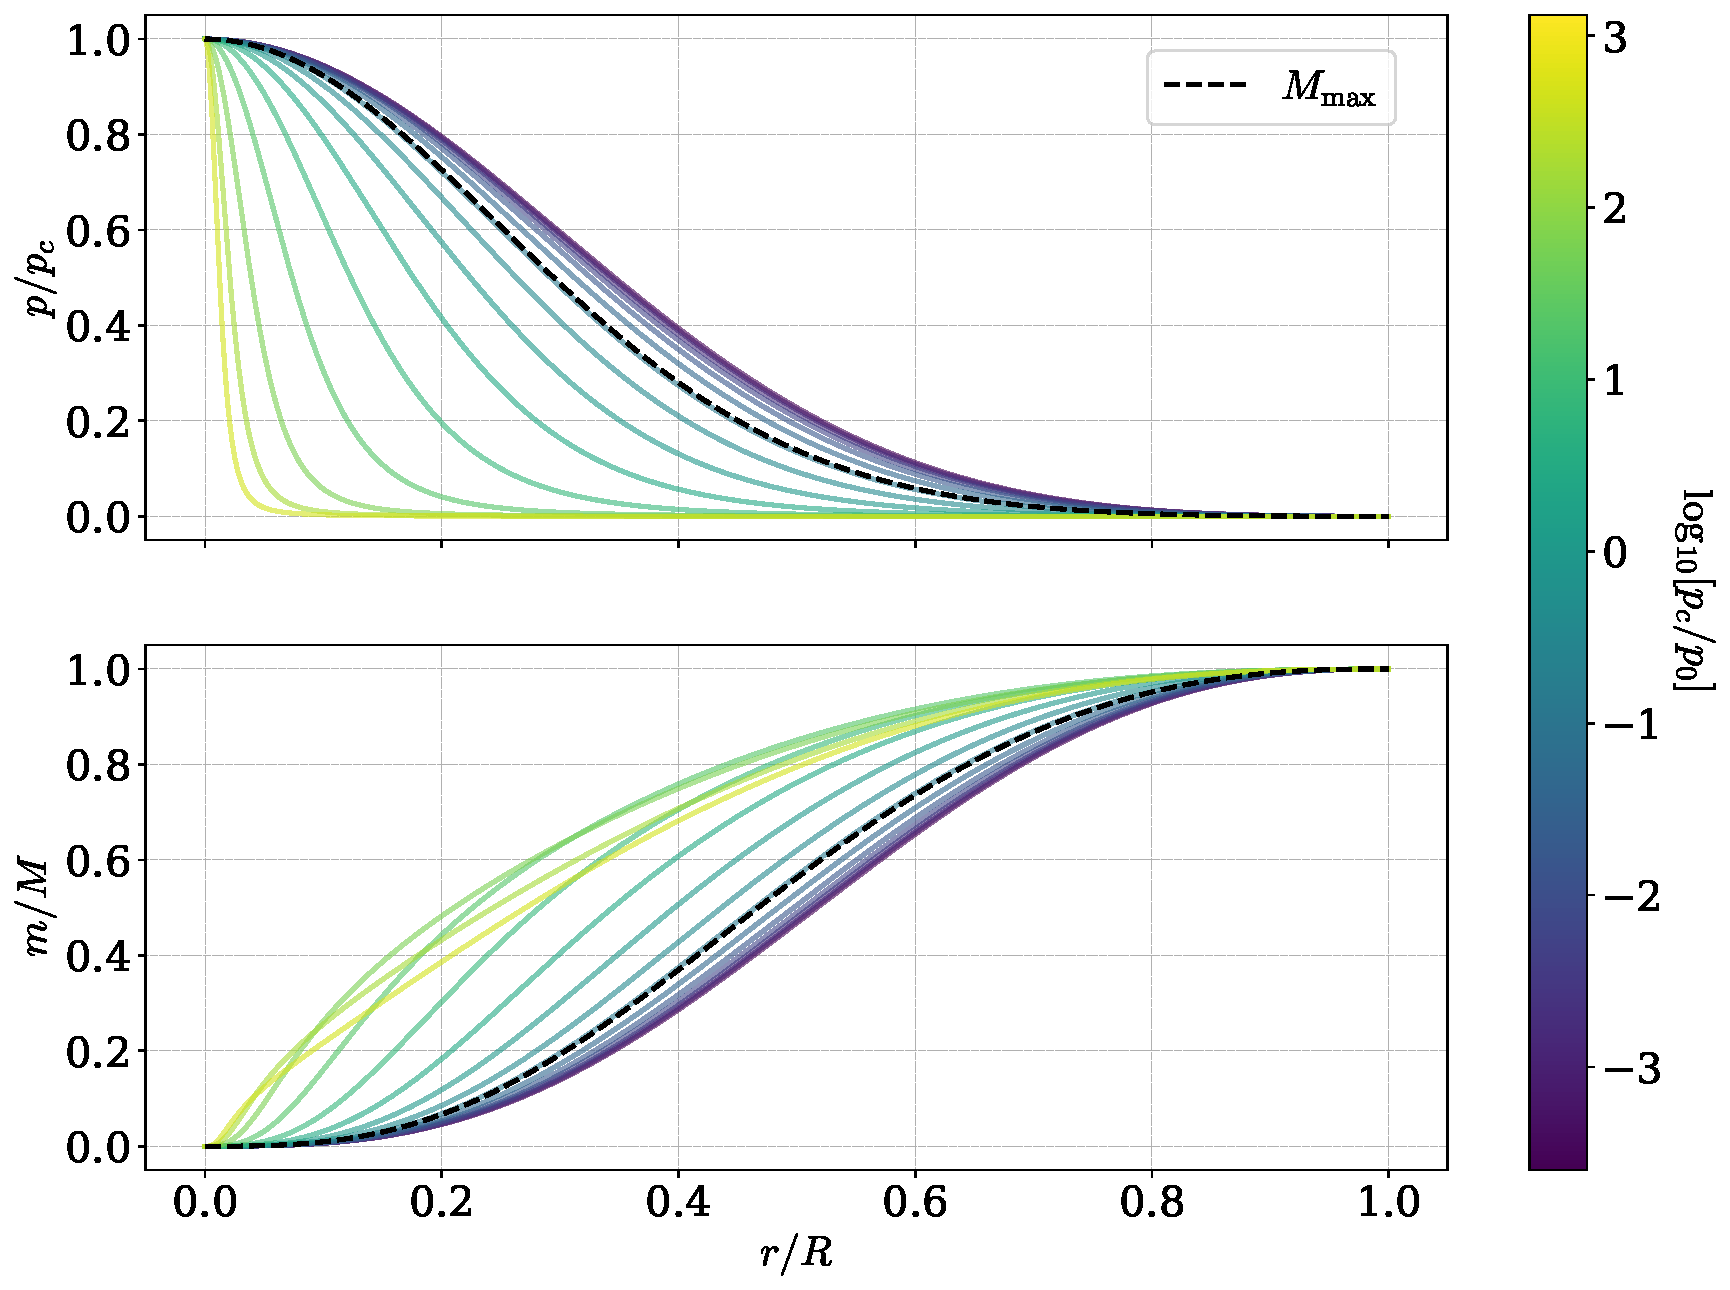
\includegraphics[width=\textwidth]{../scripts/figurer/pressure_mass.pdf}
    \caption{The pressure noramlized to central value (top) and the mass normalized to total mass (bottom), as a function of radius, nomralized to total radius. This is plotted for several different values of central pressure, which is indicated by the color shceme.}
    \label{fig: pressure and mass as a fucntion of radius}
\end{figure}


In \autoref{fig: mass radius relationship fermi gas}, we see the relationship between the mass and radius of a star made of cold Fermi gas.
This line is parameterized by the base-10 logarithm of the central pressure, $p(0)$, normalized by $p_0 = u_0$.
The cross marks the maximum mass, $M_\mathrm{max} = 0.711 \, M_\odot$, which corresponds to a radius of $R = 9.20 \, \mathrm{km}$.
This matches the results obtained by Oppenheimer and Volkoff in their 1939 paper~\cite{oppenheimerMassiveNeutronCores1939}, $M_\mathrm{max} = 0.71$.
The blue circles are the results of Oppenheimer and Volkoff paper.
\todo{Hvorfor er to punkter så langt unna?}
The black dashed line is the absolute mass-radius constraint, \autoref{mass radius constraint}, and any stable configuration must be on the right side of this line.


\begin{figure}
    \centering
    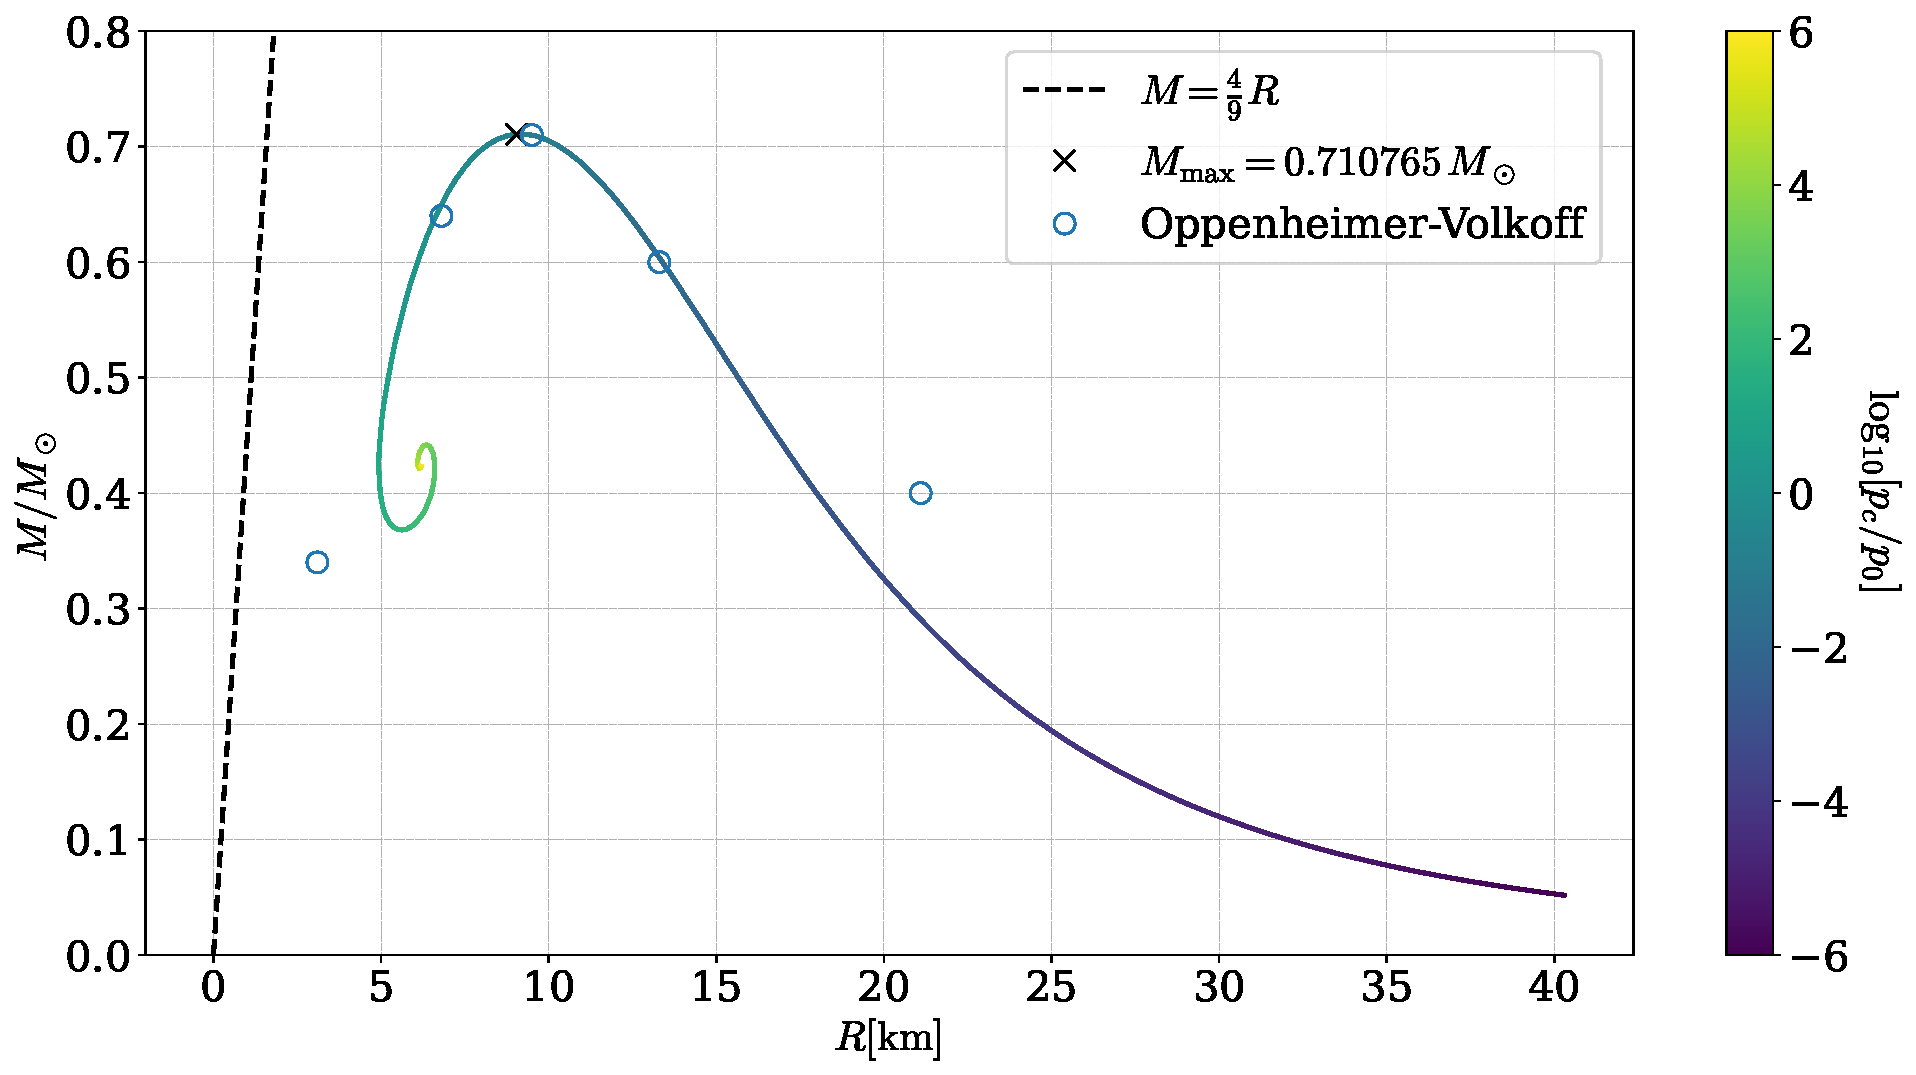
\includegraphics[width=\textwidth]{../scripts/figurer/mass_radius_neutron.pdf}
    \caption{The mass-radius relationship of a star made of a cold gas of neutrons. The line is parametrized by the boundary condition $p(0)$. The corss indicate the maximum mass solution. The blue circles are results form the 1939 paper of Oppenheimer and Volkof~\autocite{oppenheimerMassiveNeutronCores1939}.}
    \label{fig: mass radius relationship fermi gas}
\end{figure}


